% $Id$
% ..............................................................................
%                V E R S C H L U E S S E L U N G S V E R F A H R E N
%
% Schreibregelung / Syntax rules English:
%         - Chapter header with all nouns/verbs capitalized.
%         - All other headers in the normal lower/upper case manner
%           like sentences, but without dot at the end.
%
% ~~~~~~~~~~~~~~~~~~~~~~~~~~~~~~~~~~~~~~~~~~~~~~~~~~~~~~~~~~~~~~~~~~~~~~~~~~~~~~

% HACK to fix warning "destination with the same identifier .. has already been used, ...":
\makeatletter \renewcommand{\thepage}{~\csname @arabic\endcsname \c@page~} \makeatother
\hypertarget{Kapitel_1}{}
\chapter{Security Definitions and Encryption Procedures}
\label{Label_Kapitel_1}
(Bernhard Esslinger, Joerg-Cornelius Schneider, May 1999; Updates Dec. 2001, Feb. 2003, June 2005, July 2007, Jan. 2010, Mar. 2013)

This chapter introduces the topic in a more descriptive way without using too much mathematics.

The purpose of encryption \index{Encryption} is to change data in such a way
that only an authorized recipient is able to reconstruct the plaintext. This
allows us to transmit data without worrying about it getting into unauthorized
hands. Authorized recipients possess a piece of secret information -- called the
key -- which allows them to decrypt the data while it remains hidden from
everyone else.%\par \vskip + 3pt

For explanations in the following we use the notation from 
Figure \ref{Generic-Notations-when-Encrypting}:
\begin{figure}[ht]
\begin{center}
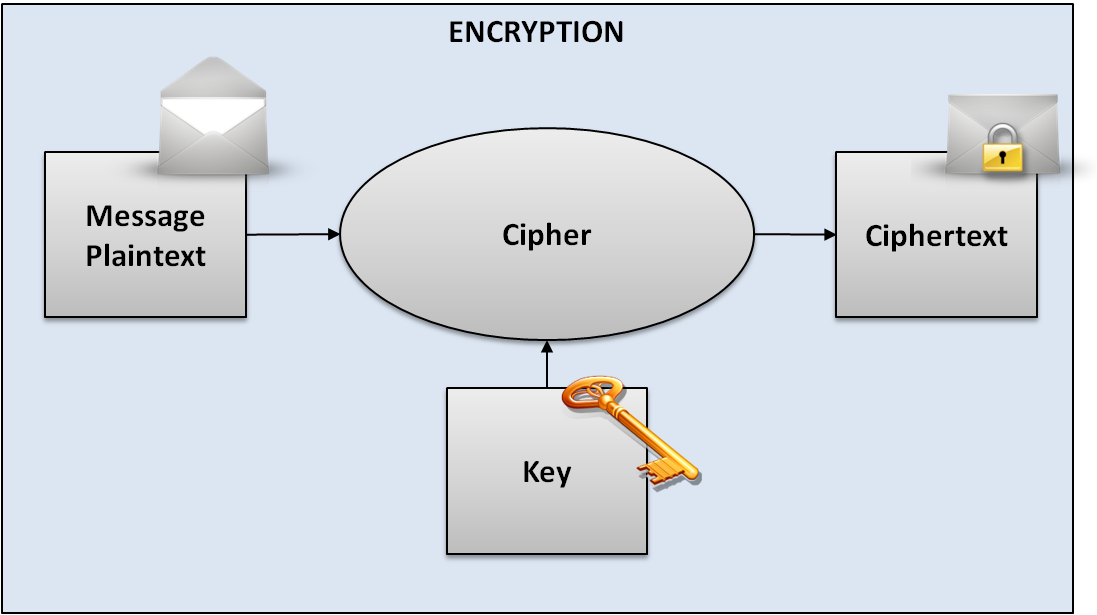
\includegraphics[scale=0.7]{figures/Generic-Notation-Encryption_en.png}
\caption{Common notations when using ciphers} 
\label{Generic-Notations-when-Encrypting}
\end{center}
\end{figure}


First we present the ideas how the security of cryptosystems is defined.



% --------------------------------------------------------------------------
\hypertarget{cm_Section_Security_Definitions}{}
\section[Security definitions]{Security definitions}
\label{cm_Section_Security_Definitions}
\index{Security definitions}

\begin{ctsquote}
\caption{Saying from India}
Explain it to me, I will forget it.\\
Show it to me, maybe I will remember it.\\
Let me do it, and I will be good at it.
\end{ctsquote}

Modern cryptography is heavily based on mathematical theory and computer
science practice. Cryptographic algorithms are designed around computational
hardness assumptions, making such algorithms hard to break in practice by any
adversary.

\vskip +3pt
Depending on the adversary's capabilities there are mainly two basic notations
of security distinguished in literature
(see e.g. {\em Contemporary Cryptography} \cite{cm:Oppliger2011}):

\begin{itemize}

\item {\bf Computational, conditional or practical security}\\
A cipher is computationally secure if it is theoretically possible to break such
a system but it is infeasible to do so by any known practical means. Theoretical
advances (e.g., improvements in integer factorization algorithms) and faster
computing technology require these solutions to be continually adapted. 

Even using the best known algorithm for breaking it will require so much
resources (e.g., 1,000,000 years) that practically the cryptosystem is secure.

So this concept is based on assumptions of the adversary's limited computing
power and the current state of science.

\item {\bf Information-theoretical or unconditional security}\\
A cipher is unconditionally secure if it is secure no matter how much resources
(time, space) the attacker has. So even in the case where an adversary has
unlimited resources for solving a problem e.g. breaking a cipher. An adversary
has not sufficient information for doing that because he is unable to gain any
meaningful data from a ciphertext.

There exist information-theoretically secure schemes that provably cannot be
broken even with unlimited computing power -- an example is the
{\em One Time Pad}\index{One Time Pad} (OTP\index{OTP}).

As the OTP is information-theoretically secure it derives its security
solely from information theory and is secure even with unlimited computing
power at the adversary's disposal. However, OTP has several practical
disadvantages (the key used must be used only once, randomly selected and must
be at least as long as the message being protected), which means that it is
hardly used except in closed environments such as for the hot wire between
Moscow and Washington.%\par \vskip + 3pt

\end{itemize}


\vskip +3pt
Two more concepts are sometimes used:

\begin{itemize}

\item {\bf Provable security}
This means that breaking such a cryptographic system is as difficult as
solving some supposedly difficult problem e.g. discrete logarithm computation,
discrete square root computation, very large integer factorization.

Example: Currently we know that RSA\index{RSA} is at most as difficult as
factorization, but we cannot prove that its exactly as difficult as
factorization.
So RSA has no proven minimum security. Or in other words: We cannot prove,
that if RSA (the cryptosystem) is broken, that then factorization (the hard
mathematical problem) can be solved.

The Rabin cryptosystem was the first cryptosystem which could be proven to be
computationally equivalent to a hard problem.

\item {\bf Ad-hoc security}
A cryptographic system has this security feature if it is not worth to try to
break into such a system because of inadequate price of data with comparison to
price of work needed to do so. Or an attack can't be done in sufficiently short
time (see {\em Handbook of Applied Cryptography} \cite{cm:Menezes2001}).

Example: This may apply if a message relevant for the stock market will be
published tomorrow and you need a year to break it.

\end{itemize}


\vskip +3pt
For good procedures used today the time taken to break them is so long that
it is practically impossible to do so, and these procedures can therefore be
considered (practically) secure -- from a pure algorithm's point of view.%\par

\vskip +3pt
We basically distinguish between symmetric and asymmetric encryption
procedures.
The book of Bruce Schneier \cite{cm:Schneier1996cm} offers a good overview of
the different encryption algorithms.
\vskip +3pt




% --------------------------------------------------------------------------
\newpage

\begin{ctsquote}
``Transparency. That's the best one can hope for in a technologically advanced society ... otherwise you will just be manipulated.''
\caption[Daniel Suarez]{Daniel Suarez\footnotemark}\index{Suarez, Daniel}
\end{ctsquote}
\addtocounter{footnote}{0}\footnotetext{Daniel Suarez, ``Freedom'',
   Dutton Adult, 2010, Chapter 5, ``Getting with the Program'', p. 63, Price.}

% --------------------------------------------------------------------------
\section[Symmetric encryption]
{Symmetric encryption\footnotemark}
  \footnotetext{%
    With CrypTool 1 ({\bf CT1})\index{CT1}\index{CrypTool 1} you can execute
    the following modern symmetric encryption algorithms 
    (using the menu path {\bf Crypt \textbackslash{} Symmetric (modern)}):\\
    IDEA, RC2, RC4, DES (ECB), DES (CBC), Triple-DES (ECB), Triple-DES (CBC),
    MARS (AES candidate), RC6 (AES candidate), Serpent (AES candidate), 
    Twofish (AES candidate), Rijndael (official AES algorithm)\index{AES}.\\
    With CrypTool 2 ({\bf CT2})\index{CT2}\index{CrypTool 2} you can execute the
    following modern symmetric encryption algorithms (using in the Startcenter
    {\bf Templates
    \textbackslash{} Cryptography \textbackslash{} Modern \textbackslash{}
    Symmetric}):\\
    AES, DES, PRESENT, RC2, RC4, SDES, TEA, Triple-DES, Twofish.\\
    In JCrypTool ({\bf JCT})\index{JCT}\index{JCrypTool} you can execute the
    following modern symmetric encryption algorithms:\\ 
    AES, Rijndael, Camellia, DES, Dragon, IDEA, LFSR, MARS, Misty1, RC2, RC5,
    RC6, SAFER+, SAFER++, Serpent, Shacal, Shacal2, Twofish.
  }

\nopagebreak
For {\em symmetric} encryption \index{Encryption!symmetric} sender and
recipient must be in possession of a common (secret) key which they have
exchanged before actually starting to communicate. The sender uses this
key to encrypt the message and the recipient uses it to decrypt it.
\par %\vskip + 3pt

This is visualized in Figure \ref{Figure_Symmetric-Enc_Secret-Key-Enc}:
\begin{figure}[ht]
\begin{center}
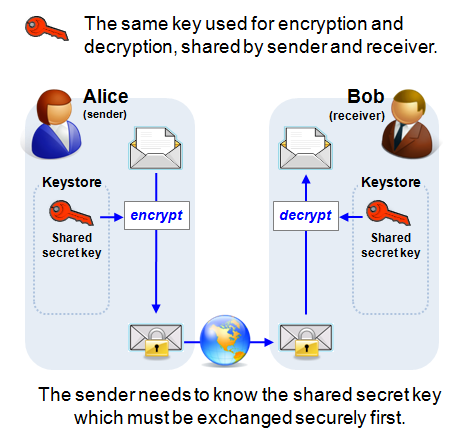
\includegraphics[scale=0.7]{figures/SymmetricEnc_Figure_Chap1_en.png}
\caption{Symmetric or Secret-Key Encryption} 
\label{Figure_Symmetric-Enc_Secret-Key-Enc}
\end{center}
\end{figure}

All classical ciphers are of the type symmetric. Examples can be found within
the CT programs, in chapter~\ref{Kapitel_PaperandPencil}
(``\nameref{Kapitel_PaperandPencil}'')
of this script, or in \cite{cm:Nichols1996}.
In this section however, we want to consider only modern symmetric mechanisms.

The advantages of symmetric algorithms are the high speed with which data can be
encrypted and decrypted. One disadvantage is the need for key management. In
order to communicate with one another confidentially, sender and recipient must
have exchanged a key using a secure channel before actually starting to
communicate. Spontaneous communication between individuals who have never met
therefore seems virtually impossible. If everyone wants to communicate with
everyone else spontaneously at any time in a network of $ n $ subscribers, each
subscriber must have previously exchanged a key with each of the other $n - 1$
subscribers. A total of $n(n - 1)/2$ keys must therefore be exchanged.\par \vskip + 3pt

The most well-known symmetric encryption procedure is the \index{DES} DES algorithm.
The DES algorithm has been developed by IBM in collaboration with the
National Security Agency \index{NSA} (NSA), and was published as a standard in
1975. Despite the fact that the procedure is relatively old, no effective attack
on it has yet been detected. The most effective way of attacking consists of
testing (almost) all possible keys until the right one is found ({\em brute-force-attack}).
\index{Attack!brute-force} Due to the relatively short key length of
effectively 56 bits (64 bits, which however include 8 parity bits), numerous
messages encrypted using DES have in the past been broken. Therefore, the
procedure can not be considered secure any longer. Alternatives to the DES
procedure include IDEA\index{IDEA}, Triple-DES and especially AES.
\par \vskip + 3pt

Up-to-the-minute procedure is the symmetric AES standard\index{AES}. The associated
Rijndael algorithm was declared winner of the AES award on October 2nd, 2000
and thus succeeds the DES procedure.\index{AES}

More details and further references about the AES algorithms and the AES
candidates of the last round can be found i.e. within the online help of
CrypTool\index{CrypTool}.%
\footnote{%
      CrypTool 1 online help\index{CrypTool 1}: The index head-word {\bf AES}
      leads to the 3 help pages: {\bf AES candidates}, 
      {\bf The AES winner Rijndael} and 
      {\bf The Rijndael encryption algorithm}\\
      A comprehensive description of AES including C code can be found
      in \cite{cm:Haan2008}.
  }


% HACK to fix warning "destination with the same identifier .. has already been used, ...":
\makeatletter \renewcommand{\thepage}{\csname @arabic\endcsname \c@page} \makeatother
% --------------------------------------------------------------------------
\subsection{Results about cryptanalysis of AES}
\label{NeueAES-Analyse}
\index{Cryptanalysis}
\index{AES}

Below you will find some results, which have recently called into question the security of the AES algorithm -- from our point of view these doubts practically still remain unfounded
% = do not bring disrepute upon AES
. 
The following information is based particularly on the original papers and the
articles \cite{cm:Wobst-iX2002} and \cite{cm:Lucks-DuD2002}.

AES with a minimum key length of 128 bit is still in the long run sufficiently secure against brute-force attacks\index{Attack!brute-force} -- as long as the quantum computers aren't powerful enough. When announced as new standard AES was immune against all known cryptanalytic attacks, mostly based on statistical considerations and earlier applied to DES: using pairs of clear and cipher texts expressions are constructed, which are not completely at random, so they allow conclusions to the used keys. These attacks required unrealistically large amounts of intercepted data.

Cryptanalysts already label methods as ``academic success'' or as ``cryptanalytic attack'' if they are theoretically faster than the complete testing of all keys (brute force analysis). In the case of AES with the maximal key length (256 bit) exhaustive key search on average needs $2^{255}$ encryption operations. A cryptanalytic attack needs to be better than this. At present between $2^{75}$ and $2^{90}$ encryption operations are estimated to be performable only just for organizations, for example a security agency.

In their 2001-paper Ferguson, Schroeppel and Whiting \cite{cm:Ferguson2001}
presented a new method of symmetric codes cryptanalysis: They described AES with
a closed formula (in the form of a continued fraction) which was possible
because of the "relatively" clear structure of AES. This formula consists of
around 1000 trillion terms of a sum - so it does not help concrete practical
cryptanalysis. Nevertheless curiosity in the academic community was awakened.
It was already known, that the 128-bit AES could be described as an
over-determined system of about 8000 quadratic equations (over an algebraic
number field) with about 1600 variables (some of them are the bits of the wanted
key) -- equation systems of that size are in practice not solvable. This special
equation system is relatively sparse, so only very few of the quadratic terms
(there are about 1,280,000 are possible quadratic terms in total) appear in the
equation system.

The mathematicians Courtois and Pieprzyk \cite{cm:Courtois2002} published a paper
in 2002, which got a great deal of attention amongst the cryptology community: The
pair had further developed the XL-method (eXtended Linearization), introduced at
Eurocrypt 2000 by Shamir et al., to create the so called XSL-method (eXtended
Sparse Linearization). The XL-method is a heuristic technique, which in some
cases manages to solve big non-linear equation systems and which was till then
used to analyze an asymmetric algorithm (HFE).  The innovation of Courtois and
Pieprzyk was, to apply the XL-method on symmetric codes: the XSL-method can be
applied to very specific equation systems. A 256-bit AES could be attacked in
roughly $2^{230}$ steps. This is still a purely academic attack, but also a
direction pointer for a complete class of block ciphers. The major problem with
this attack is that until now nobody has worked out, under what conditions it is
successful: the authors specify in their paper necessary conditions, but it is
not known, which conditions are sufficient.  There are two very new aspects of
this attack: firstly this attack is not based on statistics but on algebra. So
attacks seem to be possible, where only very small amounts of ciphertext are
available. Secondly the security of a product algorithm%
\index{Product algorithm}\index{Encryption!product algorithm}%
\index{Cascade cipher}\index{Encryption!cascade cipher}%
\footnote{%
A ciphertext can be used as input for another encryption algorithm. 
A cascade cipher%
\index{Product algorithm}\index{Encryption!product algorithm}%
\index{Cascade cipher}\index{Encryption!cascade cipher}%
is build up as a composition of different encryption transformations.
The overall cipher is called product algorithm or cascade cipher
(sometimes depending whether the used keys are statistically dependent or not).\\
Cascading does not always improve the security.\\
This process is also used {\em within} modern algorithms:
They usually combine simple and, considered at its own, cryptologically
relatively insecure single steps in several rounds into an efficient 
overall procedure.  Most block ciphers (e.g. DES, IDEA) are cascade ciphers.\\
Also serial usage of the same cipher with different keys (like with Triple-DES)
is called cascade cipher. 
}
does not exponentially increase with the number of rounds.

Currently there is a large amount of research in this area: for example Murphy and Robshaw presented a paper at Crypto 2002 \cite{cm:Robshaw2002a}, which could dramatically improve cryptanalysis: the burden for a 128-bit key was estimated at about $2^{100}$ steps by describing AES as a special case of an algorithm called BES (Big Encryption System), which has an especially "round" structure. But even $2^{100}$ steps are beyond what is achievable in the foreseeable future. Using a 256 bit key the authors estimate that a XSL-attack will require $2^{200}$ operations.

More details can be found in the Web links section at
\hyperlink{CM_HT_Weblink_Rijndael-Cryptosystem}{``AES or Rijndael cryptosystem''}.

So for AES-256 the attack is much more effective than brute-force\index{Attack!brute-force} but still far more away from any computing power which could be accessible in the short-to-long term. 

The discussion is very controversial at the moment: Don Coppersmith (one of the
inventors of DES) for example queries the practicability of the attack because
XLS would provide no solution for AES \cite{cm:Coppersmith2002}. This implies that
then the optimization of Murphy and Robshaw \cite{cm:Robshaw2002b} would not work.

In 2009 Biryukov und Khovratovich \cite{cm:Biryukov2009} published another
theoretical attack on AES. This attack uses different methods from the ones
described above. They applied methods from hash function cryptanalysis (local
collisions and boomerang switching) to construct a related-key attack on
AES-256. I.~e.\ the attacker not only needs to be able to encrypt arbitrary data
(chosen plain text), in addition he needs to be able to manipulate the unknown key
(related-key). 

Based on those assumptions, the effort to find a AES-256 key is reduced to
$2^{119}$ time and $2^{77}$ memory (considering asymmetric complexity).
In the case of AES-192 the attack is even less practical, for AES-128
the authors do not provide an attack.


% --------------------------------------------------------------------------
\subsection{Algebraic or algorithmic cryptanalysis on symmetric algorithms}
\index{Attack!algebraic}
\index{SAT solver}
\label{Algebraic-gegen-Symmetr}

There are different modern methods attacking the structure of a problem directly or after a transformation of the problem. One of the attack methods is based on the satisfiability problem (SAT)%
\footnote{%
 \url{http://en.wikipedia.org/wiki/Boolean_satisfiability_problem}
}.


%\vskip +25 pt
\paragraph*{Description of a SAT solver}\index{SAT solver}\mbox{}
\hypertarget{ht_SAT-Solver}{}

An old and well-studied problem in computer science is called the SAT problem. Here, for a given Boolean formula, it's the task to find out whether there is an assignment of the variables, so that the evaluation result of the formula is 1. 

Example: The Boolean formula "A AND B" evaluates to 1, if and only if A=B=1. For the formula "A AND NOT(A)" there exists no assignment of its variable A, so that the formula is evaluated to the value 1.

For larger Boolean formulas, it is not easy to determine if an assignment exists for which the formula can be evaluated to 1 (this problem belongs to the NP-complete problems). Therefore specific tools have been developed to solve this problem for general Boolean formulas, so called SAT solvers\footnote{
    With {\bf CT2}\index{CT2}\index{CrypTool 2} you can execute
    a SAT solver -- using in the Startcenter
    {\bf Templates
    \textbackslash{} Mathematics \textbackslash{}
    SAT Solver (Text Input)}  and  {\bf SAT Solver (File Input)}.
    }. As has been found, SAT solvers can also be used to attack cryptographic systems.


%\vskip +25 pt
\paragraph*{SAT solver based cryptanalysis}\index{SAT solver}\mbox{}
\hypertarget{ht_SAT-Solver_Cryptanalysis}{}

The general approach to use SAT solvers in cryptanalysis is very straightforward: First, the cryptographic problem, e.g. finding the symmetric key or an inversion of a hash function, is translated into a SAT problem. This is done in a way that the solution of the SAT problem solves the original cryptographic problem. Therefore, the SAT solver can be used to find a solution to the SAT problem. The paper by Massacci \cite{cm: Massacci2000} describes the first known usage of a SAT solver in this context. Unfortunately, very soon it turned out that such a general approach cannot be used efficiently in practice. This is due to the fact that the cryptographic SAT problems are very complex and the runtime of a SAT solver increases exponentially with the problem size. Therefore, in modern approaches SAT solvers are used only for solving partial problems of cryptanalysis. A good example for this is described in the paper by Mironov and Zhang \cite{cm: Mironov2006}. They demonstrate the usage of a SAT solver in an attack on hash functions, where the SAT solver is used to solve some partial problems in a very efficient way.



% --------------------------------------------------------------------------
\subsection{Current status of brute-force attacks on symmetric algorithms}
\index{Attack!brute-force}
\index{RC5}
\label{Brute-force-gegen-Symmetr}

The current status of brute-force attacks on symmetric encryption algorithms can be explained with the block cipher RC5.

Brute-force (exhaustive search, trial-and-error) means to completely examine all keys of the key space: so no special analysis methods have to be used. Instead, the ciphertext is decrypted with all possible keys%
\footnote{%
    With CT1\index{CrypTool 1} you can also perform brute-force attacks
    of modern symmetric algorithms (using the menu path
    {\bf Analysis \textbackslash{} Symmetric Encryption (modern)}): Here
    the weakest knowledge of an attacker is assumed, he performs a 
    ciphertext-only attack.\\
    With CT2\index{CrypTool 2} you can also perform brute-force attacks
    (using the templates under {\bf Cryptanalysis \textbackslash{} Modern}).
    Highly powerful is the KeySearcher component, which can be used to
    distribute the calculations to many different computers.
}
and for each resulting text it is checked, whether this is a meaningful clear text%
\footnote{%
    If the cleartext is written in a natural language and at least 100 B
    lobg, this check also can be performed automatically.\\
    To achieve a result in an appropriate time with a single PC you should 
    mark not more than 24 bit of the key as unknown.
}.
A key length of 64 bit means at most $2^{64}$ = 18,446,744,073,709,551,616 or about 18 trillion (GB) / 18 quintillion (US)  keys to check\index{CrypTool}.

Companies like RSA Security provided so-called cipher challenges in order
to quantify the security offered by well-known symmetric ciphers as DES,
Triple-DES or RC5%
\index{DES}\index{RC5}\index{Triple-DES}.%
\footnote{%
 \url{http://www.rsasecurity.com/rsalabs/challenges/secretkey/index.html}\\
 Unfortunately, in May 2007 RSA Inc announced that they will not confirm the
 correctness of the not yet solved RC5-72 challenge.}
They offered prizes for those who managed to decipher ciphertexts, encrypted with different algorithms and different key lengths, and to unveil the symmetric key (under controlled conditions). So theoretical estimates can be confirmed.

It is well-known, that the ``old'' standard algorithm DES with a fixed key
length of 56 bit is no more secure: This was demonstrated already in January
1999 by the Electronic Frontier Foundation (EFF). With their specialized
computer Deep Crack they cracked a DES encrypted message within less than a
day.\footnote{%
 \url{http://www.rsasecurity.com/rsalabs/challenges/des3/index.html}
}

The current record for strong symmetric algorithms unveiled a key 64 bit long.
The algorithm used was RC5, a block cipher with variable key size. 

The RC5-64 challenge has been solved in July 2002 by the distributed.net team
after 5 years.\footnote{%
 \url{http://www.distributed.net/Pressroom_press-rc5-64}\\
 \url{http://www.distributed.net/images/9/92/20020925_-_PR_-_64_bit_solved.pdf}
% The pdf is the former page
%  \url{http://distributed.net/pressroom/news-20020926.html}
}
In total 331,252 individuals co-operated over the internet to find the
key.\footnote{%
An overview of current distributed computing projects can be found here:\\
\url{http://distributedcomputing.info/}
}
More than 15 trillion (GB) / 15 quintillion (US)  keys were checked, until they
found the right key.

This makes clear, that symmetric algorithms (even if they have no
cryptographic weakness) using keys of size 64 bit are no more appropriate
to keep sensible data private.

There are also cipher challenges\footnote{%
  A wide spectrum of simple and complex, symmetric and asymmetric crypto riddles
  are included in the ``MysteryTwister C3''~challenge:
  \url{http://www.mysterytwisterc3.org}.
  \index{MTC3}
  \index{Challenge}
  \index{Cipher challenge}
  \index{Crypto challenge}
  }  for asymmetric algorithms (please see chapter \ref{nt:NoteFactorization}).



% --------------------------------------------------------------------------
\section[Asymmetric encryption]
{Asymmetric encryption\footnotemark}
  \footnotetext{%
    With CT1\index{CrypTool 1} you can execute RSA encryption and decryption
    (using the menu path {\bf Crypt \textbackslash{} Asymmetric}).
    In both cases you must select a RSA key pair. Only in the case of decryption
    the secret RSA key is necessary -- so here you are asked to enter the PIN.\\
    With CT2\index{CrypTool 2} you can also perform asymmetric methods
    (using the templates under {\bf Cryptography \textbackslash{} Modern}).\\
    JCT\index{JCrypTool} offers asymmetric methods like RSA both within
    the {\bf Visuals} menu of the Default Perspective as well as within the
    Algorithm Perspective.
  }
\nopagebreak
In the case of {\em asymmetric} encryption \index{Encryption!asymmetric} each
subscriber has a personal pair of keys consisting of a {\em secret}
\index{Key!secret} key and a {\em public} key\index{Key!public}. The public
key, as its name implies, is made public -- e.g. in a key directory on the
Internet (this kind of ``bill-board'' is also called just directory or
public key ring) or within a so-called public-key \index{certificate}
certificate.\par \vskip + 3pt

The asymmetric encryption is visualized in Figure \ref{Figure_Asymmetric-Enc_Public-Key-Enc}:
\begin{figure}[ht]
\begin{center}
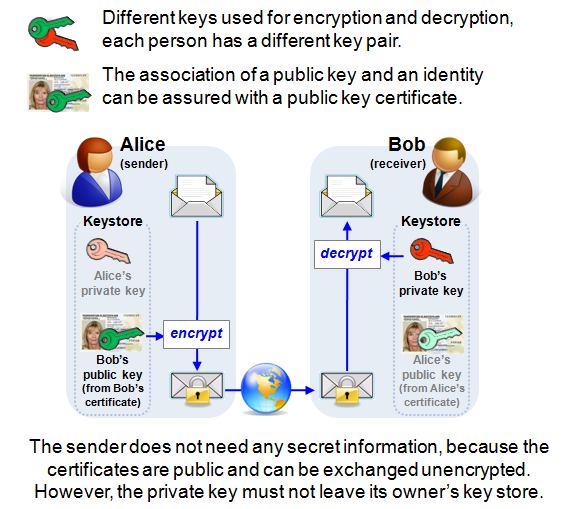
\includegraphics[scale=0.7]{figures/AsymmetricEnc_Figure_Chap1_en.png}
\caption{Asymmetric or Public-Key Encryption} 
\label{Figure_Asymmetric-Enc_Public-Key-Enc}
\end{center}
\end{figure}

If Alice\index{Alice}%
\footnote{%
      In order to describe cryptographic protocols participants
      are often named Alice, Bob\index{Bob}, \dots (see \cite[p. 23]{cm:Schneier1996cm}). 
      Alice and Bob perform all 
      2-person-protocols. Alice will initiate all protocols and 
      Bob answers. The attackers are named Eve (eavesdropper) and
      Mallory (malicious active attacker).
  } wants to communicate with Bob, then she looks for Bob's public key 
and uses it to encrypt her message to him. She then sends
this ciphertext to Bob, who is then able to decrypt it again using his 
secret key. As only Bob knows his secret key, only he can decrypt 
messages addressed to him.
Even Alice who sends the message cannot restore plaintext from the (encrypted)
message she has sent. Of course, you must first ensure that the public key
cannot be used to derive the private key.\par \vskip + 3pt

% Abbildung evtl. besser hier, wenn Seitenaufteilung ausginge.

Such a procedure can be demonstrated using a series of thief-proof letter boxes.
If I have composed a message, I then look for the letter box\index{Letter box}
of the recipient and post the letter through it. After that, I can no longer
read or change the message myself, because only the legitimate recipient has
the key for the letter box.\par \vskip + 3pt

The advantage of asymmetric procedures is the easier \index{Key management}
key management. Let's look again at a network with $n$
subscribers. In order to ensure that each subscriber can establish
an encrypted connection to each other subscriber, each subscriber
must possess a pair of keys. We therefore need $2n$ keys or $n$
pairs of keys. Furthermore, no secure channel is needed before
messages are transmitted, because all the information required in
order to communicate confidentially can be sent openly. In
this case, you simply\footnote{%
That this is also not trivial is explained e.g. in chapter
\ref{nt_Shared-Primes}.
Besides the requirements for the key generation it has to be considered that
nowadays also (public-key) infrastructures itself are targets of cyber attacks.
}
have to pay attention to the accuracy
(integrity and authenticity) \index{Authenticity} of the public
key. Disadvantage: Pure asymmetric procedures take a lot longer to
perform than symmetric ones.\par \vskip + 3pt

The most well-known asymmetric procedure is the \index{RSA} 
RSA algorithm\index{CrypTool}%
\footnote{%
The RSA algorithm is extensively described in chapter \ref{rsabeweis} and later
within this script. 
The topical research results concerning RSA are described 
in chapter \ref{SecurityRSA}.\\
The RSA cryptosystem can be executed in many variations with 
CT1\index{CrypTool 1} (using the menu path
{\bf Individual Procedures \textbackslash{} RSA Cryptosystem \textbackslash{}
RSA Demonstration}). 
}%
, named after its developers Ronald \index{Rivest, Ronald} Rivest, Adi
\index{Shamir, Adi} Shamir and Leonard \index{Adleman, Leonard} Adleman.
The RSA algorithm
was published in 1978. The concept of asymmetric encryption was first
introduced by Whitfield Diffie \index{Diffie, Whitfield}  and Martin
\index{Hellman, Martin} Hellman in 1976. Today, the ElGamal \index{ElGamal,
Tahir} procedures also play a decisive role, particularly the \index{Schnorr,
C.P.} Schnorr variant in the \index{DSA} DSA \index{Signature!digital}
(Digital Signature Algorithm).



% --------------------------------------------------------------------------
% \newpage
\section[Hybrid procedures]{Hybrid procedures\footnotemark}
\footnotetext{%
   Within CT1\index{CrypTool 1} you can find this technique using the menu
   path {\bf Crypt \textbackslash{} Hybrid}: 
   There you can follow the single steps and its dependencies with concrete
   numbers. The variant with RSA as the asymmetric algorithm is graphically
   visualized; the variant with ECC uses the standard dialogs. In both cases
   AES is used as the symmetric algorithm.\index{AES}\\
   JCT\index{JCrypTool} offers hybrid methods like ECIES within
   the Algorithm  Perspective under {\bf Algorithms \textbackslash{} Hybrid Ciphers}.
}
\label{CM_Hybrid-procedures}
\index{Hybrid procedure}

In order to benefit from the advantages of symmetric and asymmetric
techniques together, hybrid procedures \index{Encryption!hybrid} are
usually used (for encryption) in practice. \par \vskip + 3pt

In this case the bulk data is encrypted using symmetric procedures: The key
used for this is a secret session key\index{Session key} generated by the
sender randomly\footnote{%
   An important part of cryptographically secure techniques is to generate 
   random numbers. Within CT1\index{CrypTool 1} you can check out
   different random number generators using the menu path
   {\bf Indiv. Procedures \textbackslash{} Generate Random Numbers}. 
   Using the menu path {\bf Analysis \textbackslash{} Analyze Randomness}
   you can apply different test methods for random data to binary documents. \\
   CT1 concentrates on cryptographically strong {\bf pseudo} random number
   generators. ``Real'' random sources are only included via calling the
   integrated Secude generator.\\
   JCT\index{JCrypTool} offers {\bf pseudo} random number generators both
   within the Default Perspective in the menu {\bf Algorithms \textbackslash{}
   Random Number Generator} as well as within the Algorithm Perspective.
}\index{Random}
that is only used for this message.

This session key is then encrypted using the asymmetric procedure, and
transmitted to the recipient together with the message.

Recipients can determine the session key using their private keys and
then use the session key to encrypt the message.

In this way, we can benefit from the easy key management\index{Key management}
of asymmetric procedures (using public/private keys) and we benefit from the
efficiency of symmetric procedures to encrypt large quantities of data
(using secret keys).



% --------------------------------------------------------------------------
\newpage

\begin{ctsquote}
    There is an old saying inside the US National Security Agency (NSA):\\
    "Attacks always get better; they never get worse."
\caption[IETF]{IETF\footnotemark}
\end{ctsquote}
\addtocounter{footnote}{0}\footnotetext{%
  \url{http://tools.ietf.org/html/rfc4270}\index{IETF}\index{NSA}
  }

% --------------------------------------------------------------------------
\section[Cryptanalysis and symmetric ciphers for educational purposes]{Cryptanalysis and symmetric ciphers for educational purposes\footnotemark}
\footnotetext{%
A good starting point to learn cryptanalysis is the book from Mark Stamp \cite{cm:Stamp2007}.\\
Very high-level and concentrating on analysing symmetric block ciphers only is the
article from von Bruce Schneier \cite{cm:Schneier2000cm}.\\
Several of the cipher challenges at ``MysteryTwister C3''
(\url{http://www.mysterytwisterc3.org}) are also well suitable for educational purposes.
\index{MTC3}\index{Challenge}\index{Cipher challenge}\index{Crypto challenge}
}
\index{Cryptanalysis}

Compared to public-key ciphers based on mathematics like RSA, the structure of AES\index{AES} and most other modern symmetric ciphers (like DES, IDEA or Present), is very complex and cannot be explained as easily as RSA\index{RSA}.

So simplified variants of modern symmetric ciphers were developed for
educational purposes in order to allow beginners to perform
encryption and decryption by hand and gain a better understanding of how the
algorithms work in detail.
These simplified variants also help to understand and apply the according
cryptanalysis methods.

One of these variants is e.g. S-AES (Simplified-AES) by Prof. Ed Schaefer
and his students \cite{cm:Musa-etal2003}.%
\footnote{
    See the two articles with the same title
    ``Devising a Better Way to Teach and Learn the Advanced Encryption Standard''
    at the university's news at\\
    - \url{http://math.scu.edu/~eschaefe/getfile.pdf} \\
    - \url{http://www.scu.edu/cas/research/cryptography.cfm}
}
Another one is Mini-AES \cite{cm:Phan2002}
(see chapter~\ref{CM_Sage_Mini-AES} ``\nameref{CM_Sage_Mini-AES}'')%
\index{DES}\index{DES!SDES}\index{IDEA}:
\begin{itemize}

\item Edward F. Schaefer: {\em A Simplified Data Encryption Standard Algorithm} 
      \cite{cm:Schaefer1996}.

\item Raphael Chung-Wei Phan: {\em Mini Advanced Encryption Standard (Mini-AES):
                                   A Testbed for Cryptanalysis Students} 
      \cite{cm:Phan2002}.

\item Raphael Chung-Wei Phan: {\em Impossible differential cryptanalysis of Mini-AES} 
      \cite{cm:Phan2003}.

\item Mohammad A. Musa, Edward F. Schaefer, Stephen Wedig:
      {\em A simplified AES algorithm and its linear and differential cryptanalyses} 
      \cite{cm:Musa-etal2003}.

\item Nick Hoffman: {\em A SIMPLIFIED IDEA ALGORITHM} 
      \cite{cm:Hoffman2006}.

\item S. Davod. Mansoori, H. Khaleghei Bizaki: 
      {\em On the vulnerability of Simplified AES Algorithm Against Linear Cryptanalysis} 
      \cite{cm:Mansoori-etal2007}.

\end{itemize}




% --------------------------------------------------------------------------
\section{Further information}

Beside the information you can find in the following chapters, in many other
books and on a good number of websites, the online help of all
CrypTool variants\index{CrypTool} also offer very many details about the 
symmetric and asymmetric encryption methods.


	

% ---------------------------------------------------------------------------
% ---------------------------------------------------------------------------
\newpage
\hypertarget{CM_Appendix_SageCode}{}
\section{Appendix: Examples using Sage}
\label{CM_Sage_samples}
\index{Sage!Code examples}

\noindent Below is Sage source code related to contents of the
chapter~\ref{Label_Kapitel_1} (``\nameref{Label_Kapitel_1}''). 

Further details concerning cryptosystems within Sage (e.g. S-DES) can be
found e.g. in the thesis of Minh Van Nguyen \cite{cm:Nguyen2009}.

% ---------------------------------------------------------------------------
\subsection{Mini-AES}
\label{CM_Sage_Mini-AES}
\index{AES!Mini-AES}

The Sage module \texttt{crypto/block\_cipher/miniaes.py} supports Mini-AES to allow
students to explore the inner working of a modern block cipher.

Mini-AES, originally described at \cite{cm:Phan2002}, is a simplified variant of the
Advanced Encryption Standard (AES) to be used for cryptography education.

How to use Mini-AES is exhaustively described at the Sage reference page:\\
\url{http://www.sagemath.org/doc/reference/sage/crypto/block_cipher/miniaes.html}.

The following Sage code~\ref{cryptomethods:Mini-AES:Sage_example}
is taken from the release tour of Sage 4.1%
\footnote{
See \url{http://mvngu.wordpress.com/2009/07/12/sage-4-1-released/}
}
and calls the implementation of the Mini-AES.

Further example code for Mini-AES can be found in \cite[chap. 6.5 and appendix D]{cm:Nguyen2009}.

\begin{sagecode}
\begin{Verbatim}%
[fontsize=\footnotesize,fontshape=tt]
# We can encrypt a plaintext using Mini-AES as follows:
sage: from sage.crypto.block_cipher.miniaes import MiniAES
sage: maes = MiniAES()
sage: K = FiniteField(16, "x")
sage: MS = MatrixSpace(K, 2, 2)
sage: P = MS([K("x^3 + x"), K("x^2 + 1"), K("x^2 + x"), K("x^3 + x^2")]); P

[  x^3 + x   x^2 + 1]
[  x^2 + x x^3 + x^2]
sage: key = MS([K("x^3 + x^2"), K("x^3 + x"), K("x^3 + x^2 + x"), K("x^2 + x + 1")]); key

[    x^3 + x^2       x^3 + x]
[x^3 + x^2 + x   x^2 + x + 1]
sage: C = maes.encrypt(P, key); C

[            x       x^2 + x]
[x^3 + x^2 + x       x^3 + x]

# Here is the decryption process:
sage: plaintxt = maes.decrypt(C, key)
sage: plaintxt == P
True

# We can also work directly with binary strings:
sage: from sage.crypto.block_cipher.miniaes import MiniAES
sage: maes = MiniAES()
sage: bin = BinaryStrings()
sage: key = bin.encoding("KE"); key
0100101101000101
sage: P = bin.encoding("Encrypt this secret message!")
sage: C = maes(P, key, algorithm="encrypt")
sage: plaintxt = maes(C, key, algorithm="decrypt")
sage: plaintxt == P
True

# Or work with integers n such that 0 <= n <= 15:
sage: from sage.crypto.block_cipher.miniaes import MiniAES
sage: maes = MiniAES()
sage: P = [n for n in xrange(16)]; P
[0, 1, 2, 3, 4, 5, 6, 7, 8, 9, 10, 11, 12, 13, 14, 15]
sage: key = [2, 3, 11, 0]; key
[2, 3, 11, 0]
sage: P = maes.integer_to_binary(P)
sage: key = maes.integer_to_binary(key)
sage: C = maes(P, key, algorithm="encrypt")
sage: plaintxt = maes(C, key, algorithm="decrypt")
sage: plaintxt == P
True
\end{Verbatim}
\caption{Encryption and decryption with Mini-AES}
\label{cryptomethods:Mini-AES:Sage_example}
\end{sagecode}



% ---------------------------------------------------------------------------
\subsection{Further symmetric crypto algorithms in Sage}
\label{CM_Sage_SymCryptoAlg}

The Sage Reference v5.4.1%
\footnote{
See \url{http://www.sagemath.org/doc/reference/sage/crypto/}
}
lists the following further ciphers:\\ 
- Linear feedback shift register (LFSR),\\
- ShrinkingGeneratorCryptosystem,\\
- Blum-Blum-Shub (BBS) pseudorandom bit generator,\\
- Lattice related functions.




% --------------------------------------------------------------------------
\newpage
\begin{thebibliography}{99999}
\addcontentsline{toc}{section}{Bibliography}

\bibitem[Biryukov2009]{cm:Biryukov2009} \index{Biryukov 2009}
	Alex Biryukov, Dmitry Khovratovich, \\
	{\em Related-key Cryptanalysis of the Full AES-192 and AES-256},
	2009 \\
	\url{http://eprint.iacr.org/2009/317}

\bibitem[Coppersmith2002]{cm:Coppersmith2002}  \index{Coppersmith 2002}
        Don Coppersmith, \\
        {\em Re: Impact of Courtois and Pieprzyk results}, \\
        2002-09-19, ``AES Discussion Groups''~ at \\
        \url{http://aes.nist.gov/aes/}

\bibitem[Courtois2002]{cm:Courtois2002}  \index{Courtois 2002}
        Nicolas Courtois, Josef Pieprzyk, \\
        {\em Cryptanalysis of Block Ciphers with Overdefined Systems
             of Equations}, \\
        received 10 Apr 2002, last revised 9 Nov 2002.\\
        A different version, so called compact version of the first XSL attack,
        was published at Asiacrypt Dec 2002. \\
        \url{http://eprint.iacr.org/2002/044}

\bibitem[Ferguson2001]{cm:Ferguson2001}  \index{Ferguson 2001}
       Niels Ferguson, Richard Schroeppel, Doug Whiting, \\
       {\em A simple algebraic representation of Rijndael}, 
       Draft 2001/05/1, \\
       \url{http://www.xs4all.nl/~vorpal/pubs/rdalgeq.html}

\bibitem[Haan2008]{cm:Haan2008} \index{Haan 2008} 
       Kristian Laurent Haan, \\
       {\em Advanced Encryption Standard (AES)},
       2008, (German article)\\
       \url{http://www.codeplanet.eu/tutorials/cpp/51-advanced-encryption-standard.html}

\bibitem[Hoffman2006]{cm:Hoffman2006} \index{Hoffman 2006} 
       Nick Hoffman, \\
       {\em A SIMPLIFIED IDEA ALGORITHM},
       2006 \\
       \url{http://www.nku.edu/~christensen/simplified%20IDEA%20algorithm.pdf}

\bibitem[Lucks-DuD2002]{cm:Lucks-DuD2002}  \index{Lucks 2002}
       Stefan Lucks, R\"udiger Weis, \\
       {\em Neue Ergebnisse zur Sicherheit des Verschl\"usselungsstandards AES},\\
       In: DuD, Dec 2002.

\bibitem[Mansoori-etal2007]{cm:Mansoori-etal2007} \index{Mansoori, Bizaki 2007} 
       S. Davod. Mansoori, H. Khaleghei Bizaki, \\
       {\em On the vulnerability of Simplified AES Algorithm Against Linear
       Cryptanalysis}, \\
       In: IJCSNS International Journal of Computer Science and Network
       Security, Vol. 7 No. 7, July 2007, pp~257-263 \\
       See also:\\
       \url{http://paper.ijcsns.org/07_book/200707/20070735.pdf}

\bibitem[Massacci2000]{cm: Massacci2000} \index{Massacci 2000}
       Fabio Massacci, Laura Marraro \\
       {\em Logical cryptanalysis as a SAT problem: Encoding and analysis},\\ 
       In: Journal of Automated Reasoning Security,
       Vol. 24, 2000, pp~165-203.

\bibitem[Menezes2001]{cm:Menezes2001} \index{Menezes 2001}
       Alfred J. Menezes, Paul C. van Oorschot, Scott A. Vanstone \\
       {\em Handbook of Applied Cryptography}, 
       CRC Press 1997, 5th printing 2001,\\
       \url{http://www.cacr.math.uwaterloo.ca/hac/} (Errata last updated July 24, 2011).

\bibitem[Mironov2006]{cm: Mironov2006} \index{Mironov 2006}
       Ilya Mironov, Lintao Zhang \\
       {\em Applications of SAT Solvers to Cryptanalysis of Hash Functions}, 
       Springer 2006

\bibitem[Musa-etal2003]{cm:Musa-etal2003} \index{Musa, Schaefer, Wedig 2003} 
       Mohammad A. Musa, Edward F. Schaefer, Stephen Wedig, \\
       {\em A simplified AES algorithm and its linear and differential cryptanalyses}, \\
       In: Cryptologia 17 (2), April 2003, pp~148-177.\\
       See also:\\
       \url{http://findarticles.com/p/articles/mi_qa3926/is_200304/ai_n9181658}\\
       \url{http://www.rose-hulman.edu/~holden/Preprints/s-aes.pdf}\\
       \url{http://math.scu.edu/~eschaefe/}   Ed Schaefer's Homepage

\bibitem[Nguyen2009]{cm:Nguyen2009} \index{Nguyen 2009} 
       Minh Van Nguyen, \\
       {\em Exploring Cryptography Using the Sage Computer Algebra System}, \\
       Victoria University, 2009, \\
       See Sage publications \url{http://www.sagemath.org/library-publications.html},\\
       \url{http://www.sagemath.org/files/thesis/nguyen-thesis-2009.pdf},\\
       \url{http://sites.google.com/site/nguyenminh2/honours-thesis-2009.pdf}

\bibitem[Nichols1996]{cm:Nichols1996} \index{Nichols 1996} 
       Randall K. Nichols, \\
       {\em Classical Cryptography Course, Volume 1 and 2}, \\
       Aegean Park Press 1996;\\
       or in 12 lessons online at \\
       \url{http://www.fortunecity.com/skyscraper/coding/379/lesson1.htm}

\bibitem[Oppliger2011]{cm:Oppliger2011} \index{Oppliger 2011}
       Rolf Oppliger \\
       {\em Contemporary Cryptography, Second Edition},
       Artech House, 2011, \\
       \url{http://books.esecurity.ch/cryptography2e.html}.

\bibitem[Phan2002]{cm:Phan2002} \index{Phan 2002} 
       Raphael Chung-Wei Phan, \\
       {\em Mini Advanced Encryption Standard (Mini-AES): A Testbed for
            Cryptanalysis Students}, \\
       In: Cryptologia 26 (4), 2002, pp~283-306.

\bibitem[Phan2003]{cm:Phan2003} \index{Phan 2003} 
       Raphael Chung-Wei Phan, \\
       {\em Impossible differential cryptanalysis of Mini-AES}, \\
       In: Cryptologia, Oct 2003\\
       \url{http://findarticles.com/p/articles/mi_qa3926/is_200310/ai_n9311721/}

\bibitem[Robshaw2002a]{cm:Robshaw2002a}  \index{Robshaw 2002}
       S.P. Murphy, M.J.B. Robshaw, \\
       {\em Essential Algebraic Structure within the AES}, \\
       June 5, 2002, Crypto 2002,  \\
       \url{http://www.isg.rhul.ac.uk/\~{}mrobshaw/rijndael/rijndael.html}

\bibitem[Robshaw2002b]{cm:Robshaw2002b}  \index{Robshaw 2002}
       S.P. Murphy, M.J.B. Robshaw, \\
       {\em Comments on the Security of the AES and the XSL Technique}, \\
       September 26, 2002, \\
       \url{http://www.isg.rhul.ac.uk/\~{}mrobshaw/rijndael/rijndael.html}

\bibitem[Schaefer1996]{cm:Schaefer1996} \index{Schaefer 1996} 
       Edward F. Schaefer, \\
       {\em A Simplified Data Encryption Standard Algorithm}, \\
       In: Cryptologia 20 (1), 1996, pp~77-84

\bibitem[Schmeh2003]{cm:Schmeh2003}  \index{Schmeh 2003}
       Klaus Schmeh, \\
       {\em Cryptography and Public Key Infrastructures on the Internet},\\ 
       John Wiley \& Sons Ltd., Chichester 2003. \\
       An easy to read book, which also considers practical
       problems such as standardization or real existing software.
       In German, the 5th edition was published in 2013.

\bibitem[Schneier1996]{cm:Schneier1996cm} \index{Schneier 1996} 
       Bruce Schneier, \\
       {\em Applied Cryptography, Protocols, Algorithms, and Source Code in C}, \\
       Wiley 1994, 2nd edition 1996.

\bibitem[Schneier2000]{cm:Schneier2000cm} \index{Schneier 2000} 
       Bruce Schneier, \\
       {\em A Self-Study Course in Block-Cipher Cryptanalysis}, \\
       Cryptologia, v.24, Jan 2000, pp. 18-34\\
       \url{www.schneier.com/paper-self-study.pdf}

\bibitem[Stallings2006]{cm:Stallings2006} \index{Stallings 2006} 
       William Stallings, \\
       {\em Cryptography and Network Security}, \\
       Prentice Hall 2006,\\
       \url{http://williamstallings.com/}

\bibitem[Stamp2007]{cm:Stamp2007} \index{Stamp 2007} 
       Mark Stamp, Richard M. Low, \\
       {\em Applied Cryptanalysis: Breaking Ciphers in the Real World}, \\
       Wiley-IEEE Press 2007, \\
       \url{http://cs.sjsu.edu/faculty/stamp/crypto/}

\bibitem[Swenson2008]{cm:Swenson2008} \index{Swenson 2008} 
       Christopher Swenson, \\
       {\em Modern Cryptanalysis: Techniques for Advanced Code Breaking}, \\
       Wiley 2008.

\bibitem[Wobst-iX2002]{cm:Wobst-iX2002}  \index{Wobst 2002}
       Reinhard Wobst, \\
       {\em Angekratzt - Kryptoanalyse von AES schreitet voran}, \\
       In: iX, Dec 2002; \\
       plus the reader's remark by Johannes Merkle in iX Feb 2003.

\end{thebibliography}



% --------------------------------------------------------------------------
\newpage
% \section*{Web links}\addcontentsline{toc}{section}{Web links}
\chapter*{Web Links}\addcontentsline{toc}{section}{Web Links}

\begin{enumerate}

  \hypertarget{CM_HT_Weblink_Rijndael-Cryptosystem}{}
  \item AES or Rijndael cryptosystem \\
        \url{http://www.cryptosystem.net/aes}

  \item AES discussion groups at NIST \\
	\url{http://csrc.nist.gov/archive/aes/}

  \item distributed.net: ``RC5-64 has been solved'' \\
        \url{http://www.distributed.net/Pressroom_press-rc5-64}

  \item RSA: ``The RSA Secret Key Challenge'' \\
        \url{http://www.rsa.com/rsalabs/node.asp?id=2100}

  \item RSA: ``DES Challenge'' \\
        \url{http://www.rsa.com/rsalabs/node.asp?id=2108}

  \item Further links can be found at the CrypTool homepage \\
        \url{http://www.cryptool.org}
	       
\end{enumerate}

All links have been confirmed at December 12, 2012.



% Local Variables:
% TeX-master: "../script-en.tex"
% End:
